\documentclass[12pt, a4paper]{article}

% ------------------------------ font
\usepackage{times} %pdflatex
% \usepackage{luatexja}
% \usepackage{luatexja-fontspec}

% \setmainfont{Times New Roman}
% \setmainjfont[BoldFont=IPAexGothic]{IPAexMincho}
\usepackage{color}
\newcommand{\revise}[1]{{\color{red}{#1}}}

% ------------------------------ math
\usepackage{amsmath,amssymb}
\usepackage{siunitx}

% ------------------------------ author & natbib
\usepackage{authblk}
\renewcommand\Affilfont{\small}
\usepackage[semicolon]{natbib}
\bibliographystyle{agsm}

% ------------------------------ appendix
\usepackage[title]{appendix}

% ------------------------------ tables
\usepackage{here}
\usepackage{longtable, booktabs, array}
\usepackage{threeparttable, threeparttablex, multirow}
% \newcolumntype{d}{S[input-symbols = ()]}
\usepackage{lscape}

% ------------------------------- figures
\usepackage[labelfont=bf, labelsep=period, justification=justified]{caption}
\usepackage{graphics, graphicx}
\makeatletter
\def\maxwidth{\ifdim\Gin@nat@width>\linewidth\linewidth\else\Gin@nat@width\fi}
\def\maxheight{\ifdim\Gin@nat@height>\textheight\textheight\else\Gin@nat@height\fi}
\makeatother
% Scale images if necessary, so that they will not overflow the page
% margins by default, and it is still possible to overwrite the defaults
% using explicit options in \includegraphics[width, height, ...]{}
\setkeys{Gin}{width=\maxwidth,height=\maxheight,keepaspectratio}

% ------------------------------ page settings
\usepackage[left=3cm,right=3cm,top=3cm,bottom=3cm]{geometry}
\usepackage{setspace}
\renewcommand{\baselinestretch}{1.5}
\providecommand{\tightlist}{%
  \setlength{\itemsep}{0pt}\setlength{\parskip}{0pt}}

% ------------------------------ hyperlink
\usepackage[hidelinks]{hyperref}

% ------------------------------ other packages
\usepackage{booktabs}
\usepackage{siunitx}

  \newcolumntype{d}{S[
    input-open-uncertainty=,
    input-close-uncertainty=,
    parse-numbers = false,
    table-align-text-pre=false,
    table-align-text-post=false
  ]}
  

% ------------------------------ paper information
\title{Supplementary Material
``Exploring Information Provision to Promote Stem Cell Donation: Evidence from a Field Experiment of the Japan Marrow Donor Program''}
\author[a]{%
  Hiroki Kato
}
\author[b]{%
  Fumio Ohtake
}
\author[c]{%
  Saiko Kurosawa
}
\author[d]{%
  Kazuhiro Yoshiuchi
}
\author[e]{%
  Takahiro Fukuda
}
\affil[a]{School of International Politics, Economics and Communication, Aoyama Gakuin University, Tokyo, Japan}
\affil[b]{Center for Infectious Disease Education and Research (CiDER), Osaka University, Osaka, Japan}
\affil[c]{Department of Oncology, Ina Central Hospital, Nagano, Japan}
\affil[d]{Graduate School of Medicine, The University of Tokyo, Tokyo, Japan}
\affil[e]{Department of Hematopoietic Stem Cell Transplantation, National Cancer Center Hospital, Tokyo, Japan}
\date{}

\makeatletter
\renewcommand*{\@fnsymbol}[1]{\ifcase#1\or*\else\@arabic{\numexpr#1-1\relax}\fi}
\makeatother

\begin{document}
\begin{spacing}{1}
  \maketitle
  \end{spacing}



\setcounter{footnote}{0}

\tableofcontents

\appendix

\setcounter{figure}{0}
\setcounter{table}{0}
\renewcommand\thefigure{\thesection\arabic{figure}}
\renewcommand{\thetable}{\thesection\arabic{table}}
\renewcommand{\theHfigure}{\thesection\arabic{figure}}
\renewcommand{\theHtable}{\thesection\arabic{table}}

\hypertarget{figtab}{%
\section{Figures and Tables}\label{figtab}}

\begin{table}[H]

\caption{\label{tab:assignment}Assignment Schedule}
\centering
\fontsize{8}{10}\selectfont
\begin{threeparttable}
\begin{tabular}[t]{lcccccc}
\toprule
week & September, 2021 & October, 2021 & November, 2021 & December, 2021 & January, 2022 & February, 2022\\
\midrule
1 & MatchMessage & CoordMessage & CoordMessage & BothMessage & MatchMessage & StatusQuo\\
 & (09/06 to 09/12) & (10/04 to 10/10) & (11/01 to 11/07) & (11/29 to 12/05) & (01/03 to 01/09) & (01/31 to 02/06)\\
2 & BothMessage & MatchMessage & StatusQuo & StatusQuo & CoordMessage & MatchMessage\\
 & (09/13 to 09/19) & (10/11 to 10/17) & (11/08 to 11/14) & (12/06 to 12/12) & (01/10 to 01/16) & (02/07 to 02/13)\\
3 & StatusQuo & BothMessage & MatchMessage & CoordMessage & BothMessage & CoordMessage\\
 & (09/20 to 09/26) & (10/18 to 10/24) & (11/15 to 11/21) & (12/13 to 12/19) & (01/17 to 01/23) & (02/14 to 02/20)\\
4 & CoordMessage & StatusQuo & BothMessage & MatchMessage & StatusQuo & BothMessage\\
 & (09/27 to 10/03) & (10/25 to 10/31) & (11/22 to 11/28) & (12/20 to 12/26) & (01/24 to 01/30) & (02/21 to 02/27)\\
\bottomrule
\end{tabular}
\begin{tablenotes}
\item \emph{Note}: See Table 1 in the main manuscript for a detailed description of the intervention of each experimental group. The control group is the StatusQuo group. The experiment was not conducted during the week beginning December 27, 2021, and ending January 3, 2022, because JMDP was closed for the New Year's holiday.
\end{tablenotes}
\end{threeparttable}
\end{table}

\begin{table}[H]

\caption{\label{tab:smd-balance}Assessing Balance by Standardized Mean Difference}
\centering
\fontsize{8}{10}\selectfont
\begin{threeparttable}
\begin{tabular}[t]{lccc}
\toprule
\multicolumn{1}{c}{ } & \multicolumn{3}{c}{StatusQuo versus} \\
\cmidrule(l{3pt}r{3pt}){2-4}
\multicolumn{1}{c}{ } & \multicolumn{1}{c}{MatchMessage} & \multicolumn{1}{c}{CoordMessage} & \multicolumn{1}{c}{BothMessage} \\
\cmidrule(l{3pt}r{3pt}){2-2} \cmidrule(l{3pt}r{3pt}){3-3} \cmidrule(l{3pt}r{3pt}){4-4}
 & (1) & (2) & (3)\\
\midrule
Age & -0.026 & -0.096 & -0.041\\
Male (= 1) & 0.019 & 0.016 & -0.031\\
Number of holidays & 0.956 & -0.129 & 0.317\\
Number of hospitals listed with BM collection & 0.028 & 0.023 & 0.013\\
Number of hospitals listed with PBSC collection & 0.023 & 0.019 & 0.011\\
Number of listed hospitals & 0.024 & 0.019 & 0.015\\
Number of past coordinations & -0.019 & 0.015 & -0.045\\
Skipped CT (= 1) & 0.039 & 0.038 & 0.054\\
\bottomrule
\end{tabular}
\begin{tablenotes}
\item \emph{Note}: These values represent the standardized mean differences (SMD) with the control arm (experimental group A). Generally, covariates between two groups are balanced if the SMD is less than $0.1$.
\end{tablenotes}
\end{threeparttable}
\end{table}

\begin{table}[H]

\caption{\label{tab:lm-skip}Linear Probability Model of Number of Coordination and Skipping CT}
\centering
\fontsize{8}{10}\selectfont
\begin{threeparttable}
\begin{tabular}[t]{lcccccc}
\toprule
\multicolumn{1}{c}{ } & \multicolumn{3}{c}{\# Coordination $>$ 1} & \multicolumn{3}{c}{Skipped CT} \\
\cmidrule(l{3pt}r{3pt}){2-4} \cmidrule(l{3pt}r{3pt}){5-7}
  & (1) & (2) & (3) & (4) & (5) & (6)\\
\midrule
MatchMessage group & \num{-0.18} & \num{1.04} & \num{1.20} & \num{0.79} & \num{0.67} & \num{0.73}\\
 & (\num{1.94}) & (\num{1.71}) & (\num{1.87}) & (\num{0.74}) & (\num{0.69}) & (\num{0.57})\\
CoordMessage group & \num{1.69} & \num{2.04} & \num{2.05} & \num{0.76} & \num{0.50} & \num{0.54}\\
 & (\num{1.67}) & (\num{1.73}) & (\num{1.67}) & (\num{0.71}) & (\num{0.64}) & (\num{0.65})\\
BothMessage group & \num{-1.91} & \num{-1.28} & \num{-1.04} & \num{1.11} & \num{1.27} & \num{1.24}\\
 & (\num{1.90}) & (\num{1.93}) & (\num{1.92}) & (\num{1.01}) & (\num{0.94}) & (\num{0.80})\\
\midrule
Control average & 36.61 & 36.61 & 36.61 & 3.87 & 3.87 & 3.87\\
Covariates &  & X & X &  & X & X\\
Month FE &  &  & X &  &  & X\\
Num.Obs. & \num{11049} & \num{11049} & \num{11049} & \num{11049} & \num{11049} & \num{11049}\\
\bottomrule
\end{tabular}
\begin{tablenotes}
\item \emph{Note}: * $p < 0.1$, ** $p < 0.05$, *** $p < 0.01$. Standard errors clustered by the assigned week are in parentheses. The unit of treatment effect is a percentage point. Covariates are gender, age, its squared term, the number of past coordinations, the number of public holidays in the assigned week and the following week, the number of hospitals per 10 square kilometers, the number of hospitals with PBSC collection per 10 square kilometers and the number of hospitals with BM collection per 10 square kilometers. All covariates were demeaned. We excluded the number of past coordinations in model (2).
\end{tablenotes}
\end{threeparttable}
\end{table}

\begin{table}[H]

\caption{\label{tab:logit-test}Logit Model of the CT}
\centering
\fontsize{8}{10}\selectfont
\begin{threeparttable}
\begin{tabular}[t]{>{\raggedright\arraybackslash}p{20em}ccc}
\toprule
\multicolumn{1}{c}{ } & \multicolumn{3}{c}{CT} \\
\cmidrule(l{3pt}r{3pt}){2-4}
  & (1) & (2) & (3)\\
\midrule
MatchMessage group & \num{1.19} & \num{1.18} & \num{1.11}\\
 & {}[\num{1.05}, \num{1.34}] & {}[\num{1.02}, \num{1.36}] & {}[\num{0.96}, \num{1.29}]\\
CoordMessage group & \num{1.07} & \num{1.03} & \num{1.02}\\
 & {}[\num{0.94}, \num{1.22}] & {}[\num{0.90}, \num{1.19}] & {}[\num{0.89}, \num{1.17}]\\
BothMessage group & \num{1.14} & \num{1.11} & \num{1.07}\\
 & {}[\num{1.01}, \num{1.30}] & {}[\num{0.97}, \num{1.28}] & {}[\num{0.93}, \num{1.24}]\\
\midrule
Covariates &  & X & X\\
Month FE &  &  & X\\
Num.Obs. & \num{11049} & \num{11049} & \num{11049}\\
Log.Lik. & \num{-6083.783} & \num{-5306.181} & \num{-5293.272}\\
\bottomrule
\end{tabular}
\begin{tablenotes}
\item \emph{Note}: We show odds ratios and associated 95 percent confidential intervals in square brackets. Covariates are gender, age, its squared term, the number of past coordinations, the number of public holidays in the assigned week and the following week, the number of hospitals per 10 square kilometers, the number of hospitals with PBSC collection per 10 square kilometers and the number of hospitals with BM collection per 10 square kilometers. All covariates except gender dummy and dummy of skipped CT were demeaned.
\end{tablenotes}
\end{threeparttable}
\end{table}

\begin{table}[H]

\caption{\label{tab:lm-test-decompose}Decomposition of Effect on the CT}
\centering
\fontsize{8}{10}\selectfont
\begin{threeparttable}
\begin{tabular}[t]{>{\raggedright\arraybackslash}p{20em}ccccccccc}
\toprule
\multicolumn{1}{c}{ } & \multicolumn{3}{c}{Positive intention} & \multicolumn{3}{c}{No endogenous dropout} & \multicolumn{3}{c}{No exogenous dropout} \\
\cmidrule(l{3pt}r{3pt}){2-4} \cmidrule(l{3pt}r{3pt}){5-7} \cmidrule(l{3pt}r{3pt}){8-10}
  & (1) & (2) & (3) & (4) & (5) & (6) & (7) & (8) & (9)\\
\midrule
MatchMessage group & \num{2.31}* & \num{1.86}* & \num{1.27} & \num{0.97} & \num{1.14} & \num{0.93} & \num{-0.17} & \num{-0.44} & \num{-0.57}\\
 & (\num{1.33}) & (\num{1.07}) & (\num{0.93}) & (\num{1.02}) & (\num{1.09}) & (\num{0.92}) & (\num{0.83}) & (\num{0.76}) & (\num{0.51})\\
CoordMessage group & \num{-0.44} & \num{-0.05} & \num{-0.31} & \num{2.55}** & \num{1.50} & \num{1.46} & \num{-0.93} & \num{-0.96} & \num{-0.89}*\\
 & (\num{1.43}) & (\num{1.22}) & (\num{1.18}) & (\num{1.24}) & (\num{1.21}) & (\num{1.03}) & (\num{0.66}) & (\num{0.63}) & (\num{0.49})\\
BothMessage group & \num{0.59} & \num{0.24} & \num{0.12} & \num{2.27}** & \num{1.97}* & \num{1.92}* & \num{-0.51} & \num{-0.61} & \num{-0.96}**\\
 & (\num{1.61}) & (\num{1.37}) & (\num{1.09}) & (\num{1.04}) & (\num{1.14}) & (\num{1.04}) & (\num{0.72}) & (\num{0.65}) & (\num{0.42})\\
\midrule
Control average & 54.91 & 54.91 & 54.91 & 71.91 & 71.91 & 71.91 & 95.42 & 95.42 & 95.42\\
Covariates &  & X & X &  & X & X &  & X & X\\
Month FE &  &  & X &  &  & X &  &  & X\\
Num.Obs. & \num{11049} & \num{11049} & \num{11049} & \num{11049} & \num{11049} & \num{11049} & \num{11049} & \num{11049} & \num{11049}\\
\bottomrule
\end{tabular}
\begin{tablenotes}
\item \emph{Note}: * $p < 0.1$, ** $p < 0.05$, *** $p < 0.01$. The robust standard errors are in parentheses. The unit of treatment effect is a percentage point. The outcome ``No exogenous dropout'' is a dummy variable that takes a value of 1 if coordination was not interrupted due to exogenous reasons (patient-side reasons) between reply with positive intention and CT. The outcome ``No endogenous dropout'' is a dummy variable that takes a value of 1 if coordination was not interrupted due to other reasons (mainly donor-side reasons). Covariates are gender, age, its squared term, the number of past coordinations, the number of public holidays in the assigned week and the following week, the number of hospitals per 10 square kilometers, the number of hospitals with PBSC collection per 10 square kilometers, the number of hospitals with BM collection per 10 square kilometers, and a dummy indicating that candidate can have skipped the CT. All covariates except gender dummy and dummy of skipped CT were demeaned.
\end{tablenotes}
\end{threeparttable}
\end{table}

\begin{figure}[H]
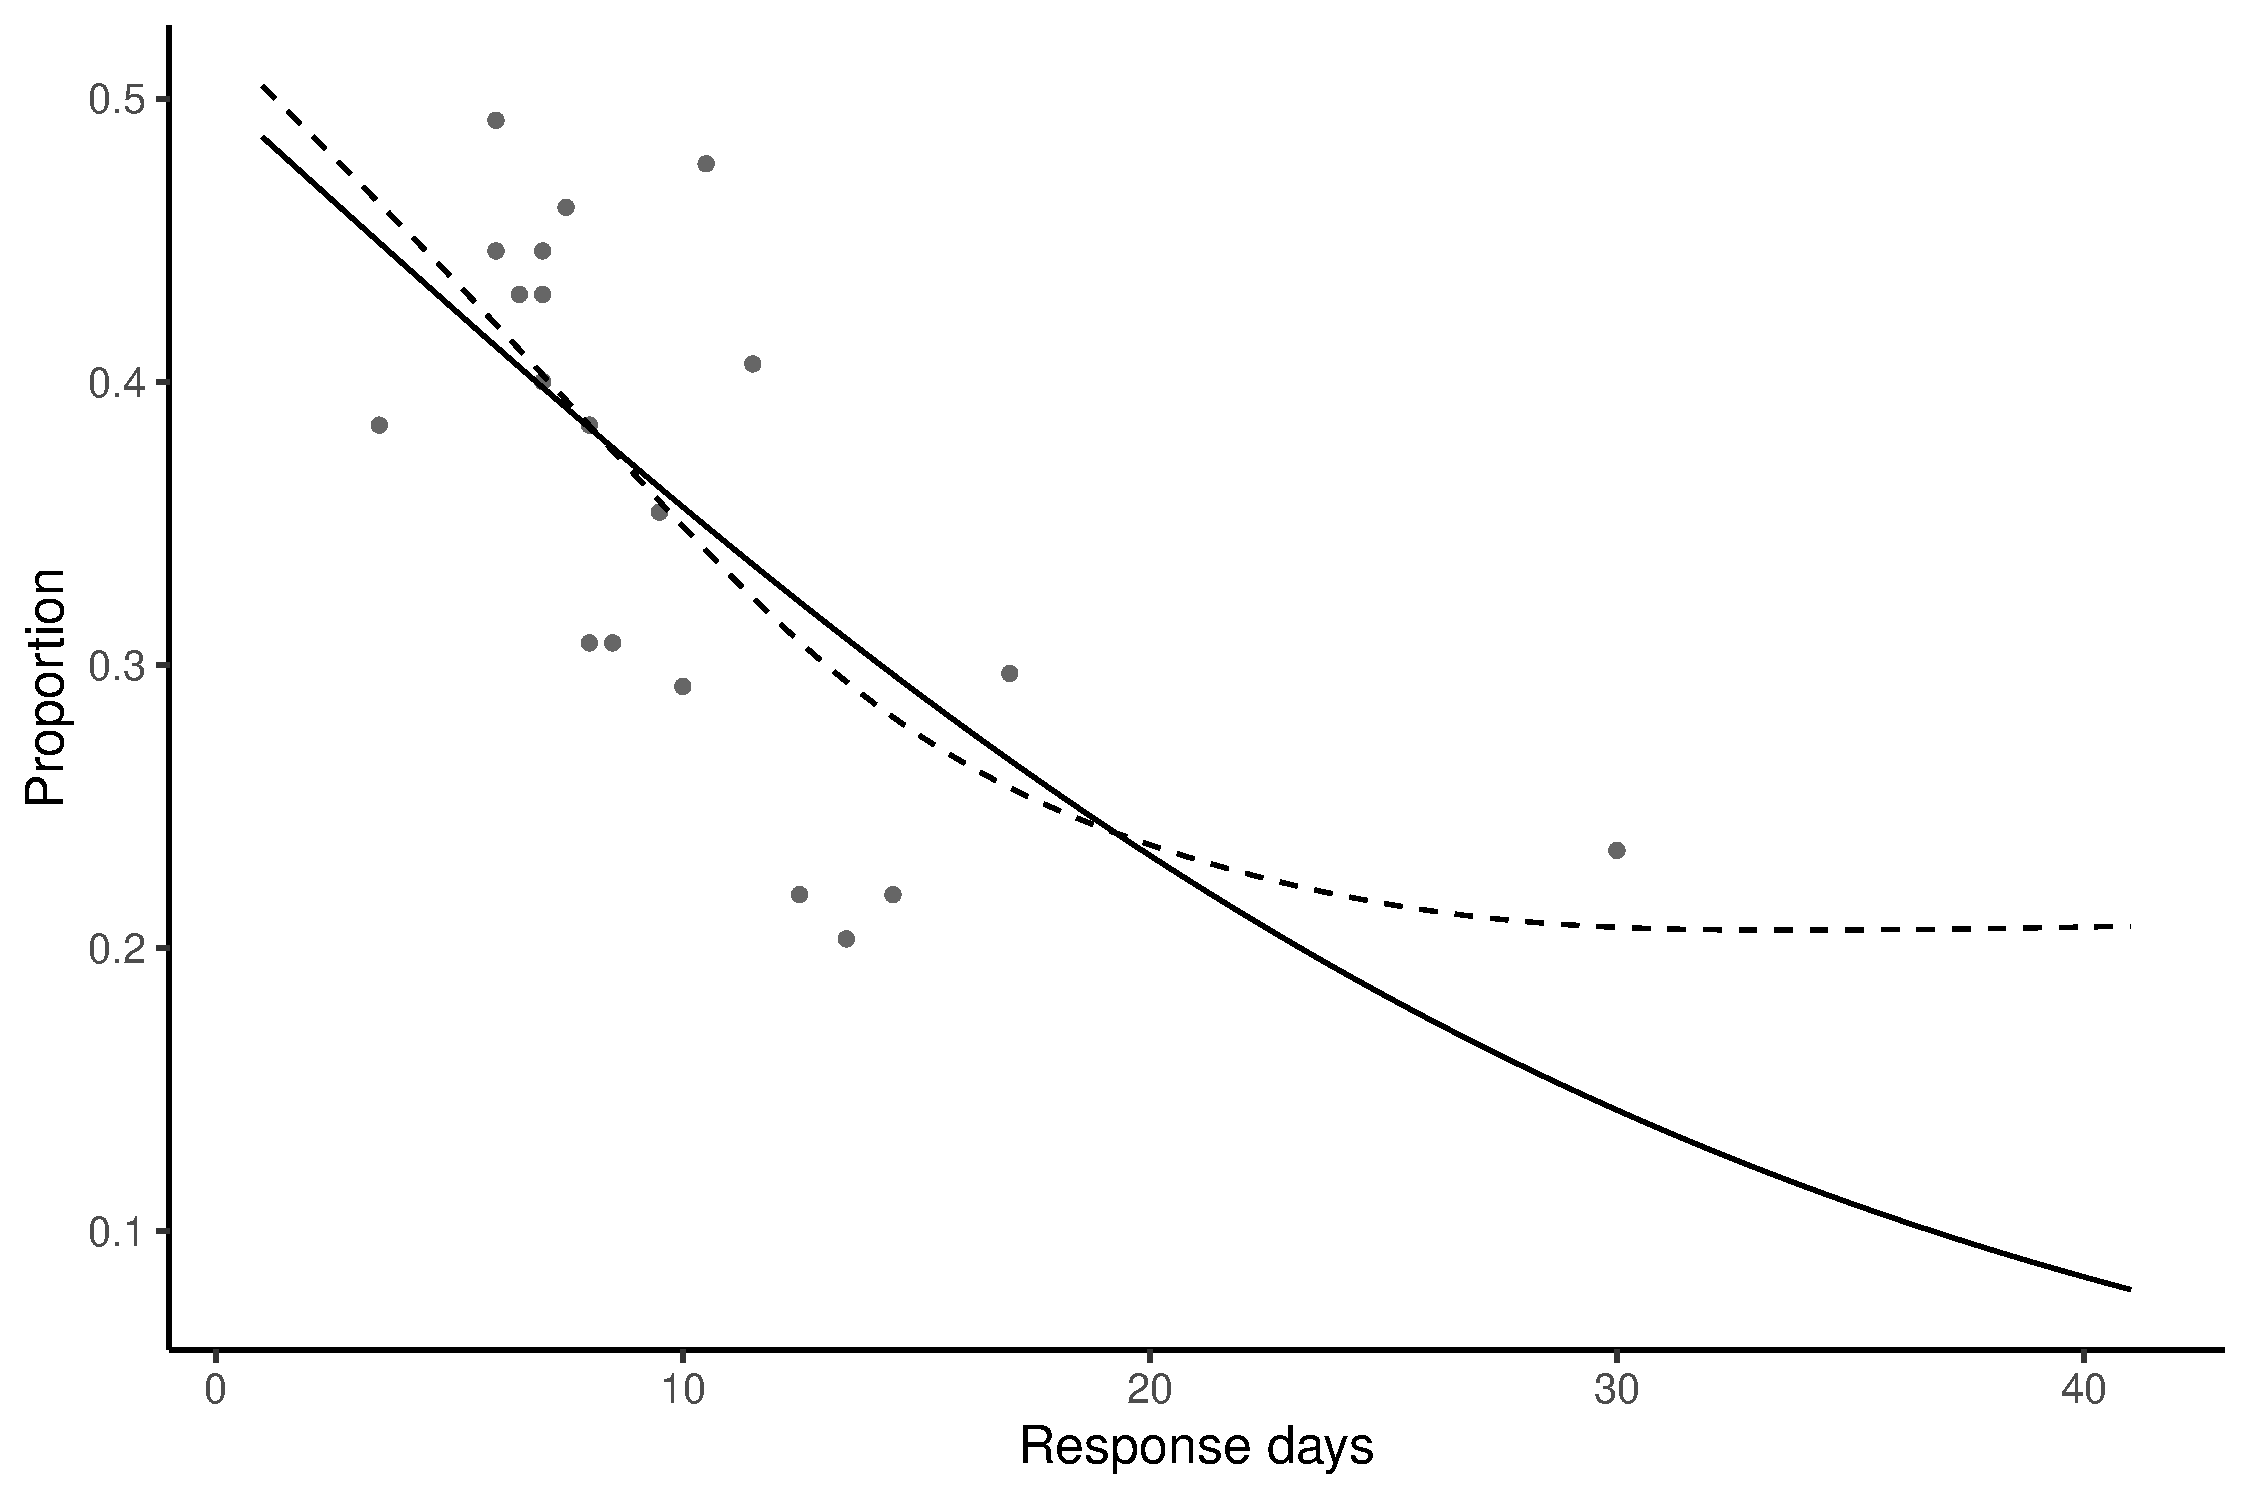
\includegraphics{JMDPRC~3/figure-latex/speed-CT-cond-response-1} \caption{Binned Scatter Plot of CT vs. Response Speed among Those Who Responded with Positive Intention. \newline \emph{Note}: We used those who responded with positive intention to donate in the control group (StatusQuo group). The dashed line represents nonparametric fitting. The solid line represents a fitted line of the logistic regression.}\label{fig:speed-CT-cond-response}
\end{figure}

\begin{figure}[H]
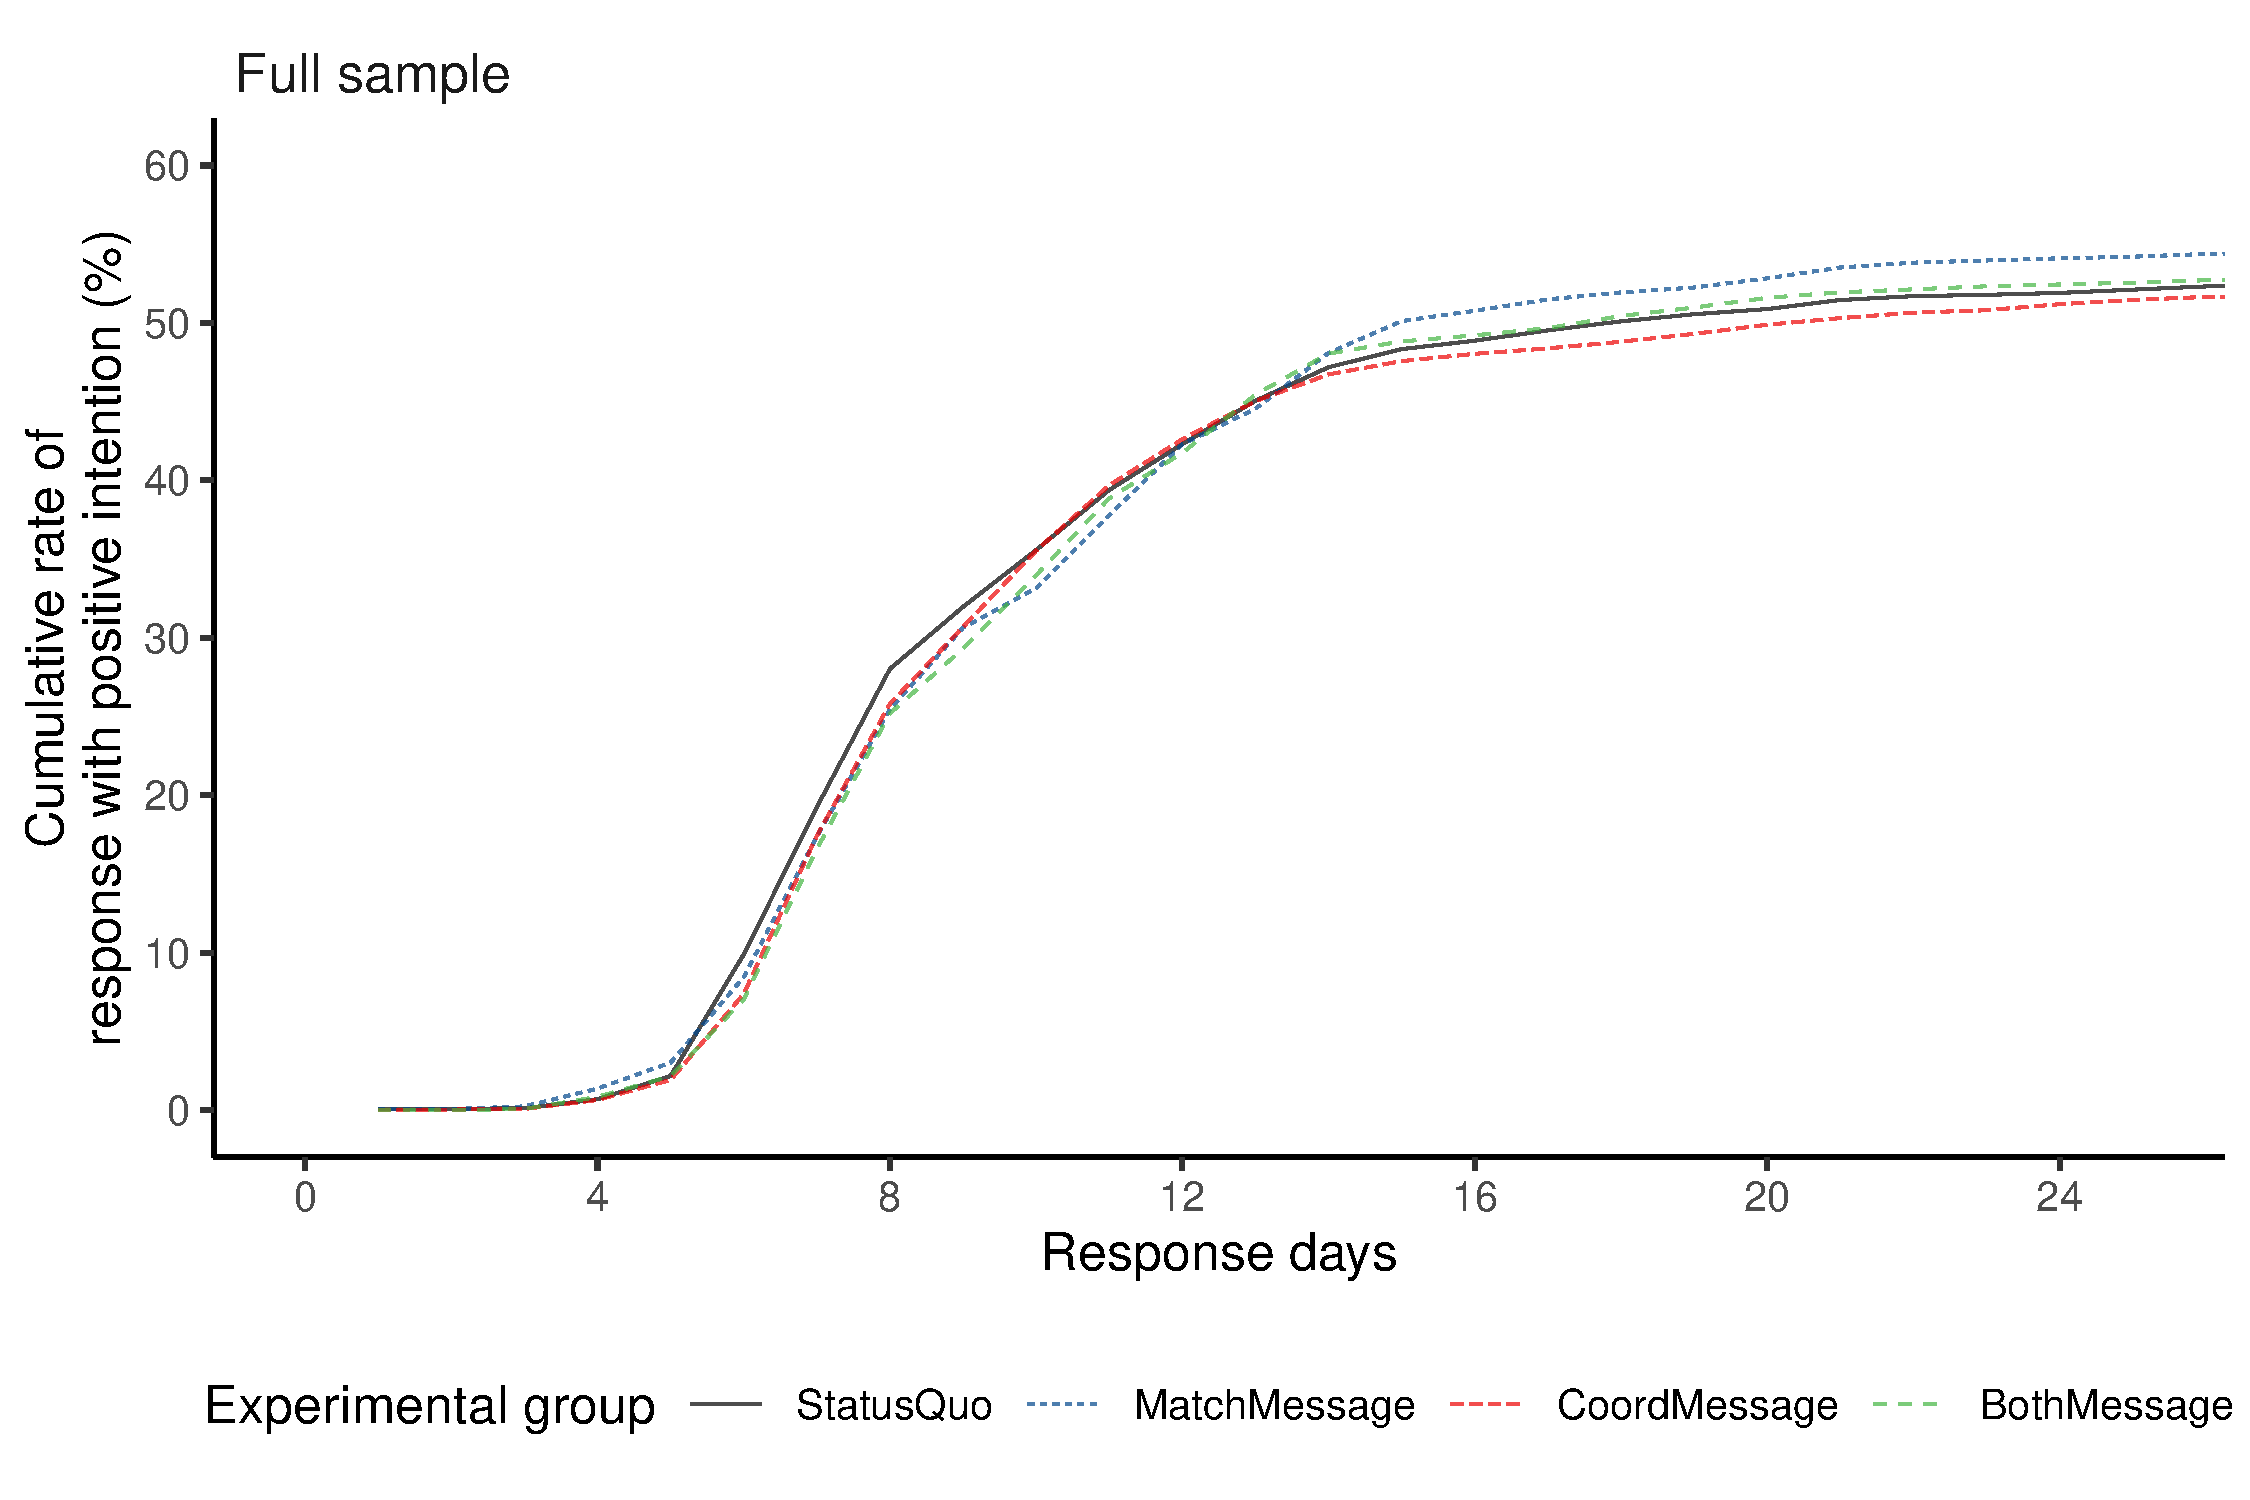
\includegraphics{JMDPRC~3/figure-latex/cumulative-response-1} \caption{Cumulative Rate of Response with Positive Intention by Treatment \newline \emph{Note}: We excluded those who skipped the CT. We only shows cumulative response rates up to 25 days after the mailing because there is no remarkable change in response rate.}\label{fig:cumulative-response}
\end{figure}

\clearpage

\begin{table}[H]

\caption{\label{tab:lm-positive-time-decompose}Effect on Speed of Response with Positive Intention}
\centering
\fontsize{8}{10}\selectfont
\begin{threeparttable}
\begin{tabular}[t]{>{\raggedright\arraybackslash}p{20em}ccccccccc}
\toprule
\multicolumn{1}{c}{ } & \multicolumn{3}{c}{0--7 days} & \multicolumn{3}{c}{8--12 days} & \multicolumn{3}{c}{13--85 days} \\
\cmidrule(l{3pt}r{3pt}){2-4} \cmidrule(l{3pt}r{3pt}){5-7} \cmidrule(l{3pt}r{3pt}){8-10}
  & (1) & (2) & (3) & (4) & (5) & (6) & (7) & (8) & (9)\\
\midrule
MatchMessage group & \num{-1.14} & \num{-0.13} & \num{-0.34} & \num{1.58} & \num{1.44} & \num{0.83} & \num{1.88} & \num{0.56} & \num{0.78}\\
 & (\num{2.39}) & (\num{3.09}) & (\num{2.47}) & (\num{1.70}) & (\num{2.14}) & (\num{2.53}) & (\num{2.17}) & (\num{1.79}) & (\num{1.14})\\
CoordMessage group & \num{-1.13} & \num{-1.47} & \num{-1.40} & \num{1.86} & \num{2.44} & \num{2.27} & \num{-1.17} & \num{-1.02} & \num{-1.18}\\
 & (\num{3.03}) & (\num{2.74}) & (\num{2.51}) & (\num{2.35}) & (\num{2.29}) & (\num{2.46}) & (\num{1.49}) & (\num{1.36}) & (\num{1.27})\\
BothMessage group & \num{-1.64} & \num{-2.15} & \num{-2.09} & \num{1.74} & \num{2.02} & \num{1.56} & \num{0.48} & \num{0.36} & \num{0.65}\\
 & (\num{2.03}) & (\num{2.44}) & (\num{2.15}) & (\num{1.87}) & (\num{1.75}) & (\num{1.89}) & (\num{1.42}) & (\num{1.49}) & (\num{1.03})\\
\midrule
Control average & 22.37 & 22.37 & 22.37 & 22.17 & 22.17 & 22.17 & 10.37 & 10.37 & 10.37\\
Covariates &  & X & X &  & X & X &  & X & X\\
Month FE &  &  & X &  &  & X &  &  & X\\
Num.Obs. & \num{11049} & \num{11049} & \num{11049} & \num{11049} & \num{11049} & \num{11049} & \num{11049} & \num{11049} & \num{11049}\\
\bottomrule
\end{tabular}
\begin{tablenotes}
\item \emph{Note}: * $p < 0.1$, ** $p < 0.05$, *** $p < 0.01$. The robust standard errors are in parentheses. The unit of treatment effect is a percentage point. The outcome is a dummy variable that takes a value of 1 if candidate responded with positive intention within a specified time after mailing. We excluded those who skipped the CT. Covariates are gender, age, its squared term, the number of past coordinations, the number of public holidays in the assigned week and the following week, the number of hospitals per 10 square kilometers, the number of hospitals with PBSC collection per 10 square kilometers and the number of hospitals with BM collection per 10 square kilometers. All covariates were demeaned.
\end{tablenotes}
\end{threeparttable}
\end{table}

\begin{figure}[H]
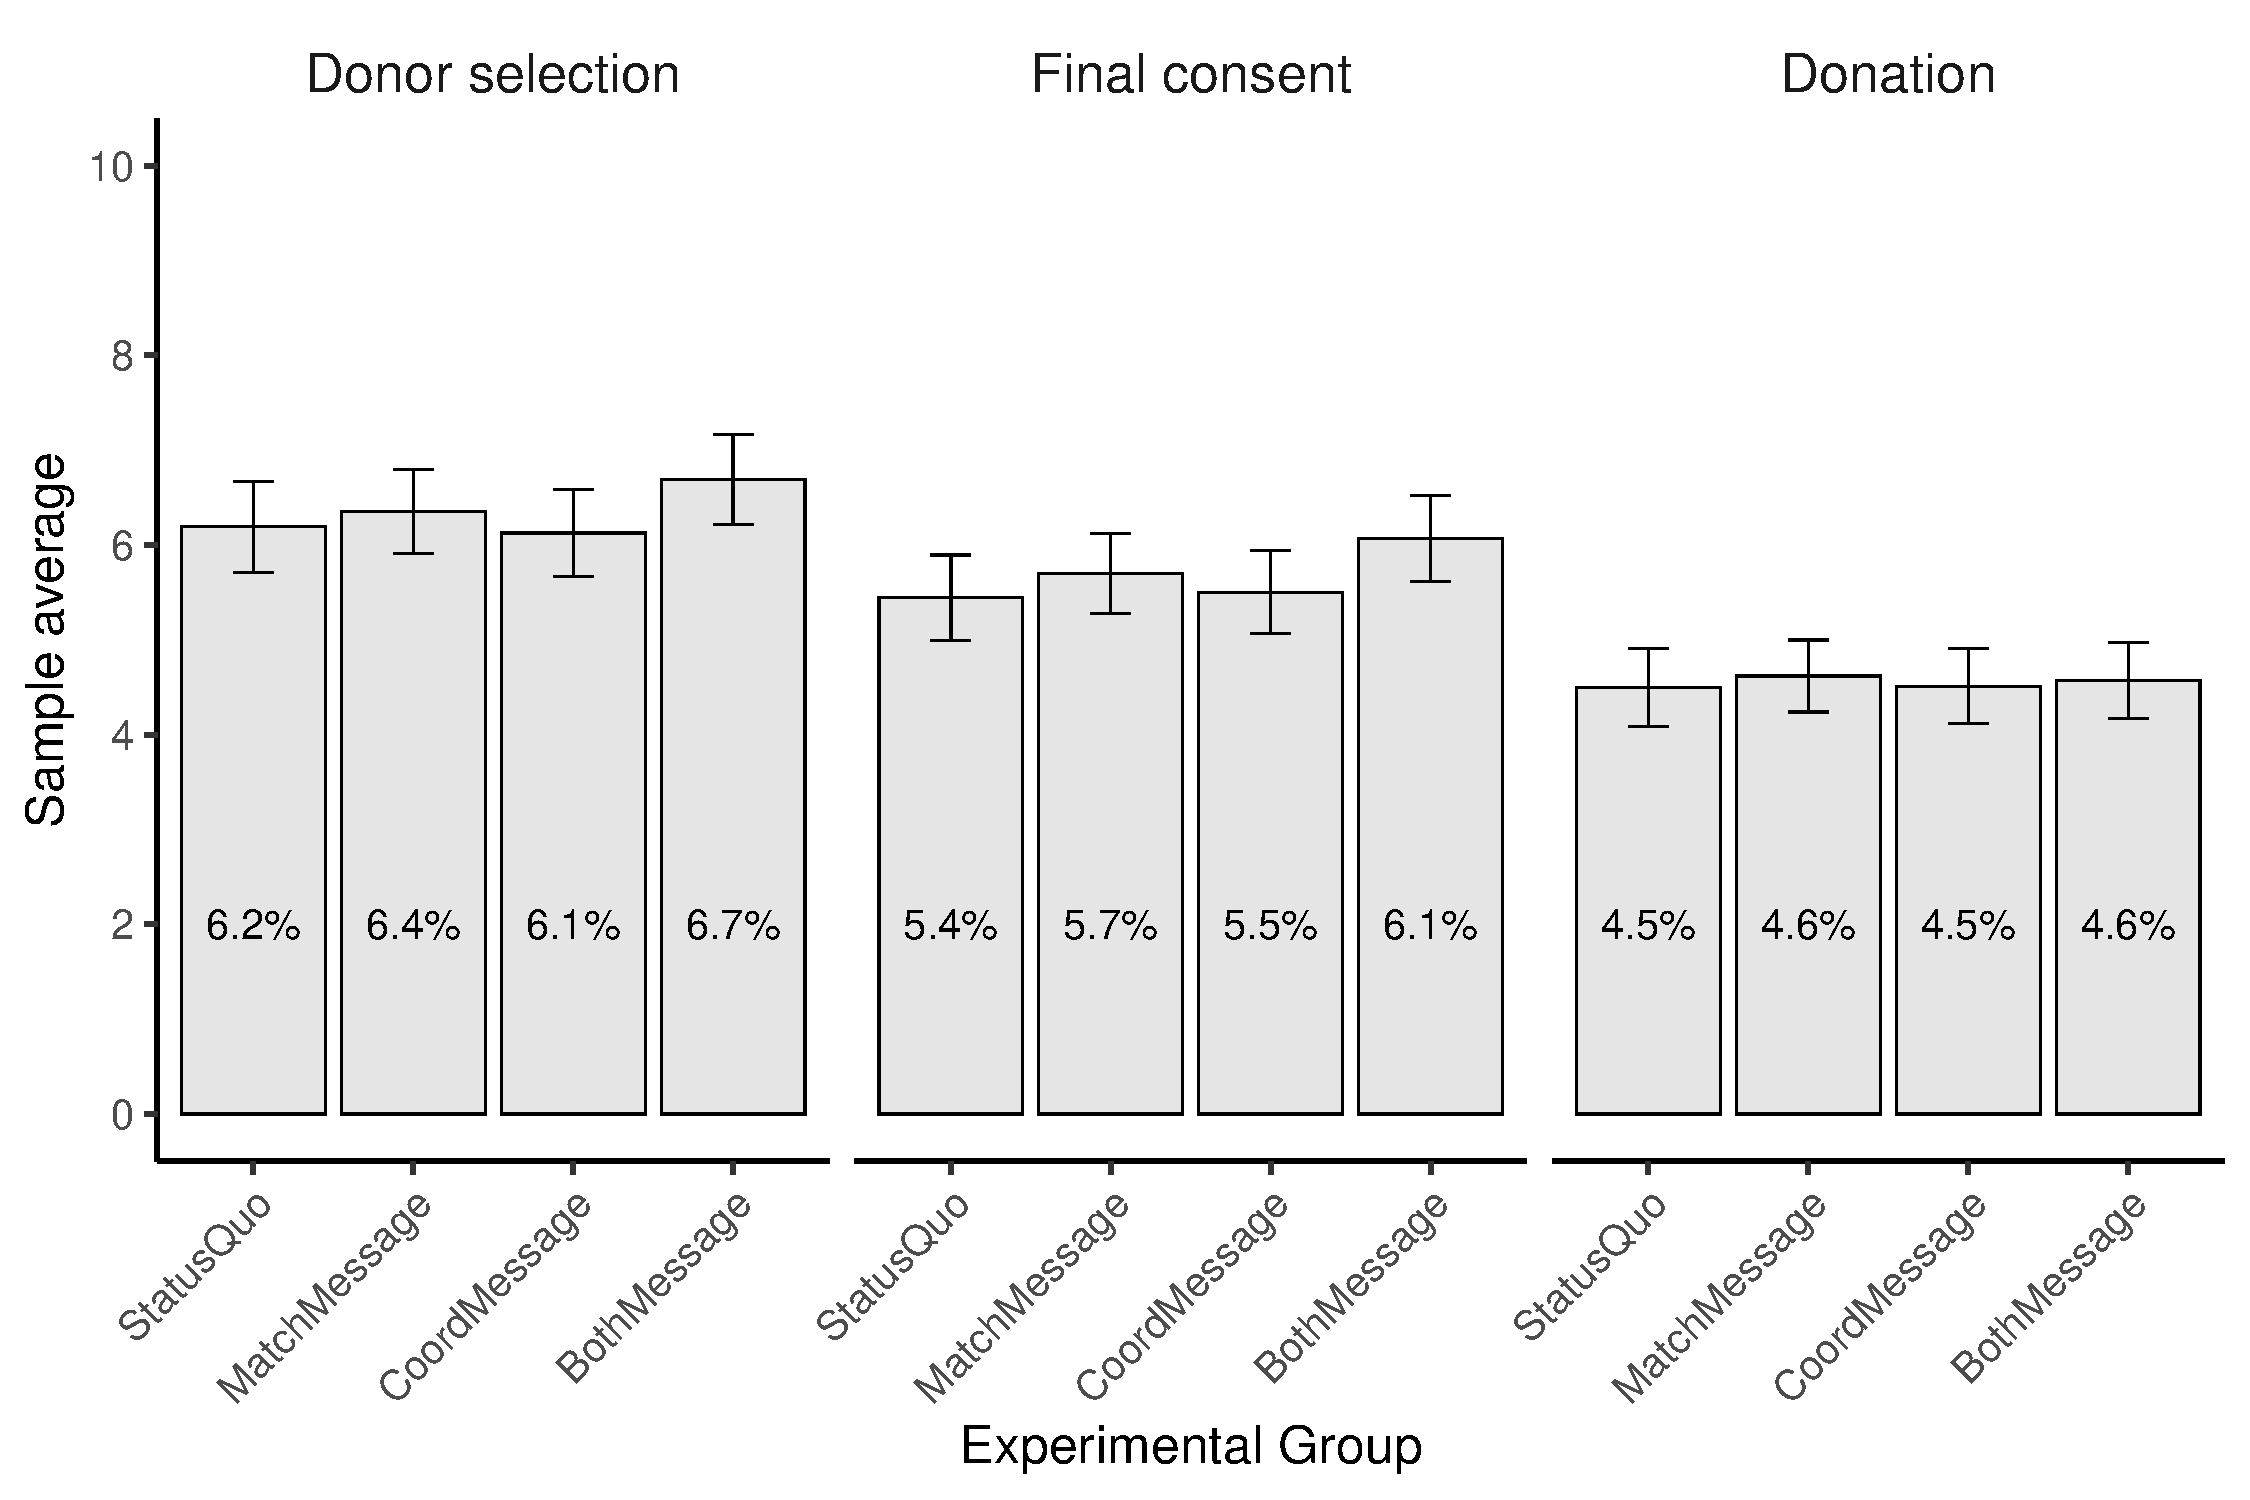
\includegraphics{JMDPRC~3/figure-latex/coordinate-diff-mean-1} \caption{Sample Averages of Donor Selection, Final Consent, and Donation by Experimental Groups.\newline \emph{Note}: Error bars show standard errors of the mean. For the statistical test, we used standard errors clustered by the assigned week.}\label{fig:coordinate-diff-mean}
\end{figure}

\begin{table}[H]

\caption{\label{tab:lm-coordinate}Linear Probability Model of the Coordination Processes After CT}
\centering
\fontsize{8}{10}\selectfont
\begin{threeparttable}
\begin{tabular}[t]{lccccccccc}
\toprule
\multicolumn{1}{c}{ } & \multicolumn{3}{c}{Donor selection} & \multicolumn{3}{c}{Final consent} & \multicolumn{3}{c}{Donation} \\
\cmidrule(l{3pt}r{3pt}){2-4} \cmidrule(l{3pt}r{3pt}){5-7} \cmidrule(l{3pt}r{3pt}){8-10}
  & (1) & (2) & (3) & (4) & (5) & (6) & (7) & (8) & (9)\\
\midrule
MatchMessage group & \num{0.16} & \num{-0.29} & \num{-0.71}** & \num{0.26} & \num{-0.14} & \num{-0.58}** & \num{0.12} & \num{-0.12} & \num{-0.48}\\
 & (\num{0.59}) & (\num{0.56}) & (\num{0.35}) & (\num{0.56}) & (\num{0.51}) & (\num{0.28}) & (\num{0.45}) & (\num{0.47}) & (\num{0.37})\\
CoordMessage group & \num{-0.07} & \num{-0.32} & \num{-0.39} & \num{0.06} & \num{-0.16} & \num{-0.22} & \num{0.02} & \num{-0.15} & \num{-0.20}\\
 & (\num{0.76}) & (\num{0.70}) & (\num{0.37}) & (\num{0.64}) & (\num{0.58}) & (\num{0.31}) & (\num{0.57}) & (\num{0.52}) & (\num{0.33})\\
BothMessage group & \num{0.50} & \num{0.26} & \num{0.00} & \num{0.63} & \num{0.43} & \num{0.19} & \num{0.07} & \num{-0.08} & \num{-0.28}\\
 & (\num{0.72}) & (\num{0.81}) & (\num{0.35}) & (\num{0.80}) & (\num{0.88}) & (\num{0.42}) & (\num{0.74}) & (\num{0.80}) & (\num{0.50})\\
\midrule
Control average & 6.19 & 6.19 & 6.19 & 5.44 & 5.44 & 5.44 & 4.50 & 4.50 & 4.50\\
Covariates &  & X & X &  & X & X &  & X & X\\
Month FE &  &  & X &  &  & X &  &  & X\\
Num.Obs. & \num{11049} & \num{11049} & \num{11049} & \num{11049} & \num{11049} & \num{11049} & \num{11049} & \num{11049} & \num{11049}\\
\bottomrule
\end{tabular}
\begin{tablenotes}
\item \emph{Note}: * $p < 0.1$, ** $p < 0.05$, *** $p < 0.01$. Standard errors clustered by the assigned week are in parentheses. The unit of treatment effect is a percentage point. Covariates are sex, (demeaned) age, its squared term, the number of past coordinations, the number of public holidays in the assigned week and following week, the number of hospitals per 10 square kilometers, the number of hospitals with PBSC collection per 10 square kilometers, and the number of hospitals with bone marrow collection per 10 square kilometers. All the covariates except sex were demeaned.
\end{tablenotes}
\end{threeparttable}
\end{table}

\clearpage

\begin{landscape}\begin{table}[H]

\caption{\label{tab:logit-coordinate}Logit Model of Coordination Process After CT}
\centering
\fontsize{8}{10}\selectfont
\begin{threeparttable}
\begin{tabular}[t]{lccccccccc}
\toprule
\multicolumn{1}{c}{ } & \multicolumn{3}{c}{Donor selection} & \multicolumn{3}{c}{Final consent} & \multicolumn{3}{c}{Donation} \\
\cmidrule(l{3pt}r{3pt}){2-4} \cmidrule(l{3pt}r{3pt}){5-7} \cmidrule(l{3pt}r{3pt}){8-10}
  & (1) & (2) & (3) & (4) & (5) & (6) & (7) & (8) & (9)\\
\midrule
MatchMessage group & \num{1.03} & \num{0.95} & \num{0.89} & \num{1.05} & \num{0.98} & \num{0.90} & \num{1.03} & \num{0.97} & \num{0.90}\\
 & {}[\num{0.83}, \num{1.28}] & {}[\num{0.75}, \num{1.21}] & {}[\num{0.70}, \num{1.14}] & {}[\num{0.83}, \num{1.32}] & {}[\num{0.76}, \num{1.26}] & {}[\num{0.70}, \num{1.17}] & {}[\num{0.80}, \num{1.32}] & {}[\num{0.74}, \num{1.29}] & {}[\num{0.68}, \num{1.19}]\\
CoordMessage group & \num{0.99} & \num{0.96} & \num{0.95} & \num{1.01} & \num{0.99} & \num{0.98} & \num{1.00} & \num{0.98} & \num{0.97}\\
 & {}[\num{0.79}, \num{1.24}] & {}[\num{0.76}, \num{1.21}] & {}[\num{0.75}, \num{1.20}] & {}[\num{0.80}, \num{1.28}] & {}[\num{0.77}, \num{1.26}] & {}[\num{0.77}, \num{1.25}] & {}[\num{0.77}, \num{1.30}] & {}[\num{0.75}, \num{1.27}] & {}[\num{0.74}, \num{1.26}]\\
BothMessage group & \num{1.09} & \num{1.06} & \num{1.02} & \num{1.12} & \num{1.10} & \num{1.06} & \num{1.02} & \num{0.99} & \num{0.96}\\
 & {}[\num{0.87}, \num{1.35}] & {}[\num{0.84}, \num{1.32}] & {}[\num{0.81}, \num{1.28}] & {}[\num{0.89}, \num{1.42}] & {}[\num{0.87}, \num{1.39}] & {}[\num{0.83}, \num{1.35}] & {}[\num{0.78}, \num{1.32}] & {}[\num{0.76}, \num{1.29}] & {}[\num{0.73}, \num{1.25}]\\
\midrule
Covariates &  & X & X &  & X & X &  & X & X\\
Month FE &  &  & X &  &  & X &  &  & X\\
Num.Obs. & \num{11049} & \num{11049} & \num{11049} & \num{11049} & \num{11049} & \num{11049} & \num{11049} & \num{11049} & \num{11049}\\
Log.Lik. & \num{-2610.914} & \num{-2464.319} & \num{-2454.591} & \num{-2410.035} & \num{-2283.231} & \num{-2272.377} & \num{-2045.363} & \num{-1954.414} & \num{-1944.719}\\
\bottomrule
\end{tabular}
\begin{tablenotes}
\item \emph{Note}: We show odds ratios and associated 95 percent confidential intervals in square brackets. Covariates are gender, age, its squared term, the number of past coordinations, the number of public holidays in the assigned week and the following week, the number of hospitals per 10 square kilometers, the number of hospitals with PBSC collection per 10 square kilometers and the number of hospitals with BM collection per 10 square kilometers. All covariates except gender dummy and dummy of skipped CT were demeaned.
\end{tablenotes}
\end{threeparttable}
\end{table}
\end{landscape}

\clearpage

\begin{table}[H]

\caption{\label{tab:lm-interaction-gender-test-donate}Heterogenous Message Effects on CT and Donation by Gender}
\centering
\fontsize{8}{10}\selectfont
\begin{threeparttable}
\begin{tabular}[t]{>{\raggedright\arraybackslash}p{30em}cccccc}
\toprule
\multicolumn{1}{c}{ } & \multicolumn{3}{c}{CT} & \multicolumn{3}{c}{Donation} \\
\cmidrule(l{3pt}r{3pt}){2-4} \cmidrule(l{3pt}r{3pt}){5-7}
  & (1) & (2) & (3) & (4) & (5) & (6)\\
\midrule
MatchMessage group & \num{2.73}* & \num{1.90} & \num{0.91} & \num{-0.47} & \num{-0.77}* & \num{-1.10}*\\
 & (\num{1.44}) & (\num{1.67}) & (\num{1.36}) & (\num{0.43}) & (\num{0.43}) & (\num{0.57})\\
CoordMessage group & \num{1.60} & \num{-1.02} & \num{-1.45} & \num{0.24} & \num{-0.12} & \num{-0.24}\\
 & (\num{1.52}) & (\num{1.57}) & (\num{1.21}) & (\num{0.66}) & (\num{0.69}) & (\num{0.48})\\
BothMessage group & \num{4.91}*** & \num{2.74} & \num{2.03} & \num{-0.43} & \num{-0.80} & \num{-1.06}**\\
 & (\num{1.51}) & (\num{1.93}) & (\num{1.50}) & (\num{0.44}) & (\num{0.54}) & (\num{0.47})\\
Male & \num{4.58}** & \num{3.37}** & \num{3.21}** & \num{2.17}*** & \num{2.32}*** & \num{2.27}***\\
 & (\num{1.88}) & (\num{1.50}) & (\num{1.58}) & (\num{0.67}) & (\num{0.73}) & (\num{0.74})\\
MatchMessage group $\times$ Male & \num{0.52} & \num{1.04} & \num{1.10} & \num{0.90} & \num{1.07} & \num{1.01}\\
 & (\num{2.18}) & (\num{1.96}) & (\num{2.01}) & (\num{0.79}) & (\num{0.94}) & (\num{0.96})\\
CoordMessage group $\times$ Male & \num{-0.71} & \num{2.38}* & \num{2.68}* & \num{-0.38} & \num{0.03} & \num{0.13}\\
 & (\num{1.93}) & (\num{1.44}) & (\num{1.51}) & (\num{0.83}) & (\num{0.84}) & (\num{0.83})\\
BothMessage group $\times$ Male & \num{-4.01} & \num{-1.92} & \num{-1.63} & \num{0.89} & \num{1.19} & \num{1.30}\\
 & (\num{2.60}) & (\num{2.34}) & (\num{2.40}) & (\num{0.92}) & (\num{0.91}) & (\num{0.89})\\
\midrule
\addlinespace[0.3em]
\multicolumn{7}{l}{\textit{Linear combination test: Experimental group + Experimental group $\times$ Male}}\\
\hspace{1em}MatchMessage group & 3.25* & 2.94** & 2.01* & 0.43 & 0.30 & -0.08\\
\hspace{1em} & (1.90) & (1.48) & (1.09) & (0.64) & (0.76) & (0.60)\\
\hspace{1em}CoordMessage group & 0.90 & 1.36 & 1.23 & -0.14 & -0.09 & -0.11\\
\hspace{1em} & (1.96) & (1.27) & (1.12) & (0.72) & (0.63) & (0.54)\\
\hspace{1em}BothMessage group & 0.89 & 0.82 & 0.40 & 0.45 & 0.39 & 0.24\\
\hspace{1em} & (2.33) & (2.05) & (1.35) & (1.06) & (1.08) & (0.75)\\
\hspace{1em}Covariates &  & X & X &  & X & X\\
Month FE &  &  & X &  &  & X\\
Num.Obs. & \num{11049} & \num{11049} & \num{11049} & \num{11049} & \num{11049} & \num{11049}\\
\bottomrule
\end{tabular}
\begin{tablenotes}
\item \emph{Note}: * $p < 0.1$, ** $p < 0.05$, *** $p < 0.01$. The robust standard errors are in parentheses. This table tests heterogenous message effects by gender. The unit of treatment effect is a percentage point. Covariates are age, the number of past coordinations, the number of public holidays in the assigned week and the following week, the number of hospitals per 10 square kilometers, the number of hospitals with PBSC collection per 10 square kilometers and the number of hospitals with BM collection per 10 square kilometers. All covariates were demeaned. We also controlled cross terms of each covariate and gender.
\end{tablenotes}
\end{threeparttable}
\end{table}

\begin{table}[H]

\caption{\label{tab:lm-interaction-coordination1-test-donate}Heterogeneous Treatment Effects on CT and Donation by First-Time Coordination}
\centering
\fontsize{8}{10}\selectfont
\begin{threeparttable}
\begin{tabular}[t]{>{\raggedright\arraybackslash}p{30em}cccccc}
\toprule
\multicolumn{1}{c}{ } & \multicolumn{3}{c}{CT} & \multicolumn{3}{c}{Donation} \\
\cmidrule(l{3pt}r{3pt}){2-4} \cmidrule(l{3pt}r{3pt}){5-7}
  & (1) & (2) & (3) & (4) & (5) & (6)\\
\midrule
MatchMessage group & \num{4.20} & \num{3.91}* & \num{2.98}* & \num{-0.14} & \num{0.39} & \num{0.00}\\
 & (\num{3.08}) & (\num{2.37}) & (\num{1.75}) & (\num{0.95}) & (\num{0.78}) & (\num{0.88})\\
CoordMessage group & \num{4.02} & \num{2.70} & \num{2.46} & \num{0.04} & \num{-0.19} & \num{-0.26}\\
 & (\num{3.16}) & (\num{2.37}) & (\num{2.11}) & (\num{0.86}) & (\num{0.76}) & (\num{0.78})\\
BothMessage group & \num{3.80} & \num{0.95} & \num{0.57} & \num{0.30} & \num{-0.10} & \num{-0.26}\\
 & (\num{3.41}) & (\num{2.60}) & (\num{1.82}) & (\num{1.01}) & (\num{1.20}) & (\num{0.99})\\
First-time coordination & \num{-9.78}*** & \num{-1.07} & \num{-1.00} & \num{-1.92}* & \num{0.35} & \num{0.35}\\
 & (\num{2.89}) & (\num{2.11}) & (\num{2.17}) & (\num{0.99}) & (\num{1.21}) & (\num{1.22})\\
MatchMessage group $\times$ First-time coordination & \num{-1.69} & \num{-2.19} & \num{-2.16} & \num{0.41} & \num{-0.80} & \num{-0.76}\\
 & (\num{3.10}) & (\num{2.28}) & (\num{2.35}) & (\num{1.38}) & (\num{1.31}) & (\num{1.31})\\
CoordMessage group $\times$ First-time coordination & \num{-4.86} & \num{-3.62} & \num{-3.59} & \num{-0.09} & \num{0.05} & \num{0.08}\\
 & (\num{3.31}) & (\num{2.56}) & (\num{2.62}) & (\num{1.08}) & (\num{0.98}) & (\num{0.99})\\
BothMessage group $\times$ First-time coordination & \num{-1.86} & \num{0.94} & \num{0.72} & \num{-0.28} & \num{0.02} & \num{-0.04}\\
 & (\num{3.67}) & (\num{2.27}) & (\num{2.32}) & (\num{1.27}) & (\num{1.16}) & (\num{1.19})\\
\midrule
\addlinespace[0.3em]
\multicolumn{7}{l}{\textit{Linear combination test: Experimental group + Experimental group $\times$ First-Time Coordination}}\\
\hspace{1em}MatchMessage group & 2.51*** & 1.72 & 0.82 & 0.27 & -0.41 & -0.76\\
\hspace{1em} & (0.79) & (1.05) & (1.01) & (0.69) & (0.79) & (0.64)\\
\hspace{1em}CoordMessage group & -0.83 & -0.92 & -1.13 & -0.05 & -0.14 & -0.18\\
\hspace{1em} & (1.15) & (1.12) & (1.09) & (0.69) & (0.66) & (0.42)\\
\hspace{1em}BothMessage group & 1.94 & 1.89 & 1.30 & 0.01 & -0.08 & -0.31\\
\hspace{1em} & (1.61) & (1.49) & (1.01) & (0.94) & (0.84) & (0.60)\\
\hspace{1em}Covariates &  & X & X &  & X & X\\
Month FE &  &  & X &  &  & X\\
Num.Obs. & \num{11049} & \num{11049} & \num{11049} & \num{11049} & \num{11049} & \num{11049}\\
\bottomrule
\end{tabular}
\begin{tablenotes}
\item \emph{Note}: * $p < 0.1$, ** $p < 0.05$, *** $p < 0.01$. The robust standard errors are in parentheses. The unit of treatment effect is a percentage point. Covariates are age, its squared term, the number of public holidays in the assigned week and the following week, the number of hospitals per 10 square kilometers, the number of hospitals with PBSC collection per 10 square kilometers and the number of hospitals with BM collection per 10 square kilometers. All covariates were demeaned. We also controlled cross terms of each covariate and dummy of first-time coordination.
\end{tablenotes}
\end{threeparttable}
\end{table}

\begin{table}[H]

\caption{\label{tab:lm-who-selected}Determination of Donor Selection}
\centering
\fontsize{8}{10}\selectfont
\begin{threeparttable}
\begin{tabular}[t]{lcccccc}
\toprule
\multicolumn{1}{c}{ } & \multicolumn{6}{c}{Donor selection} \\
\cmidrule(l{3pt}r{3pt}){2-7}
  & (1) & (2) & (3) & (4) & (5) & (6)\\
\midrule
(Intercept) & \num{38.53}*** & \num{19.85} & \num{30.94}** & \num{12.68} &  & \\
 & (\num{8.33}) & (\num{30.13}) & (\num{14.84}) & (\num{32.18}) &  & \\
Male & \num{8.76}** & \num{8.71}** & \num{8.22}** & \num{8.16}** & \num{8.17}** & \num{8.10}**\\
 & (\num{3.93}) & (\num{3.93}) & (\num{3.96}) & (\num{3.96}) & (\num{3.98}) & (\num{3.98})\\
Age & \num{-0.34}* & \num{0.75} & \num{-0.33}* & \num{0.73} & \num{-0.37}* & \num{0.92}\\
 & (\num{0.20}) & (\num{1.68}) & (\num{0.20}) & (\num{1.68}) & (\num{0.20}) & (\num{1.70})\\
Age (squared) &  & \num{-0.01} &  & \num{-0.01} &  & \num{-0.02}\\
 &  & (\num{0.02}) &  & (\num{0.02}) &  & (\num{0.02})\\
\# coordination experiences & \num{-1.83} & \num{-1.94}* & \num{-1.92}* & \num{-2.03}* & \num{-1.81} & \num{-1.93}*\\
 & (\num{1.16}) & (\num{1.16}) & (\num{1.15}) & (\num{1.16}) & (\num{1.15}) & (\num{1.15})\\
\# holidays &  &  & \num{1.76} & \num{1.76} & \num{9.64}*** & \num{4.10}\\
 &  &  & (\num{2.69}) & (\num{2.70}) & (\num{2.32}) & (\num{7.78})\\
\# listed hospitals &  &  & \num{14.22} & \num{14.53} & \num{17.86} & \num{18.35}\\
 &  &  & (\num{16.20}) & (\num{16.19}) & (\num{16.34}) & (\num{16.34})\\
\# listed hospitals with PBSC collection &  &  & \num{-8.52} & \num{-7.57} & \num{-3.93} & \num{-2.60}\\
 &  &  & (\num{31.89}) & (\num{31.92}) & (\num{32.34}) & (\num{32.36})\\
\# listed hospitals with BM collection &  &  & \num{-22.78} & \num{-23.74} & \num{-31.86} & \num{-33.35}\\
 &  &  & (\num{37.39}) & (\num{37.34}) & (\num{37.76}) & (\num{37.74})\\
\midrule
Num.Obs. & \num{564} & \num{564} & \num{564} & \num{564} & \num{564} & \num{564}\\
R2 & \num{0.016} & \num{0.017} & \num{0.020} & \num{0.021} & \num{0.026} & \num{0.027}\\
R2 Adj. & \num{0.011} & \num{0.009} & \num{0.008} & \num{0.007} & \num{0.006} & \num{0.006}\\
Month FE &  &  &  &  & X & X\\
\bottomrule
\end{tabular}
\begin{tablenotes}
\item \emph{Note}: * $p < 0.1$, ** $p < 0.05$, *** $p < 0.01$. The robust standard errors are in parentheses. The unit of coefficients is a percentage point. We used potential donors who completed the CT in the control arm. The number of holidays is the sum of the number of holidays in the assigned week and the following week. The number of listed hospitals is per 10 square kilometers.
\end{tablenotes}
\end{threeparttable}
\end{table}

\begin{spacing}{1}
  \bibliography{biblio.bib}
\end{spacing}


\end{document}
